%Preamble
\documentclass[newPxFont]{beamer}
\usetheme{sthlm}
%\usecolortheme{sthlmv42}
%-=-=-=-=-=-=-=-=-=-=-=-=-=-=-=-=-=
%        Packages
%-=-=-=-=-=-=-=-=-=-=-=-=-=-=-=-=-=
\usepackage[utf8]{inputenc}
\usepackage{chronology}
\usepackage{hyperref}
\usepackage{amsmath}
\usepackage{amssymb}
\usepackage{booktabs}
%----------------------------------
%Comandos:
\newcommand \imageFrame[2]{
\begingroup
\begin{frame}
  \begin{center}
\includegraphics[width=4in]{#1}\\
\Large #2
    \end{center}
\end{frame}
\endgroup
}

\renewcommand{\event}[3][e]{%
  \pgfmathsetlength\xstop{(#2-\theyearstart)*\unit}%
  \ifx #1e%
    \draw[fill=black,draw=none,opacity=0.5]%
      (\xstop, 0) circle (.2\unit)%
      node[opacity=1,rotate=45,right=.2\unit] {#3};%
  \else%
    \pgfmathsetlength\xstart{(#1-\theyearstart)*\unit}%
    \draw[fill=black,draw=none,opacity=0.5,rounded corners=.1\unit]%
      (\xstart,-.1\unit) rectangle%
      node[opacity=1,rotate=45,right=.2\unit] {#3} (\xstop,.1\unit);%
  \fi}%
%-=-=-=-=-=-=-=-=-=-=-=-=-=-=-=-=-=-=-
%        Beamer options
%-=-=-=-=-=-=-=-=-=-=-=-=-=-=-=-=-=-=-
%\setbeameroption{show notes}
%-=-=-=-=-=-=-=-=-=-=-=-=-=-=-=-=-=-=-
%        PGFPlots options
%-=-=-=-=-=-=-=-=-=-=-=-=-=-=-=-=-=-=-
%\pgflotsset{compat=1.14}

%-=-=-=-=-=-=-=-=-=-=-=-=-=-=-=-=-=-=-
%
%	Information
%
%-=-=-=-=-=-=-=-=-=-=-=-=-=-=-=-=-=-=-
\title{Biomedical Engineering Summer School, Wilhelmshaven 2018}
\subtitle{ Instrumentation, Acquisition and Signal Processing for Biosignals}
%\date{\small{\jobname}}
\date{\today}
\author{\texttt{Gerardo Marx Chávez-Campos\\ Mehmet Y\"uksekkaya}}
\institute{\textit{Instituto Tecnológico de Morelia}}

\hypersetup{
pdfauthor = {Marx: gmarx-cc@itmorelia.edu.mx},
pdfsubject = {Fourier series},
pdfkeywords = {orthogonal function, },
pdfmoddate= {D:\pdfdate},
pdfcreator = {Chavez-Campos}
}

\begin{document}
%Title:
\maketitle
%\begin{frame}[plain]
%	\titlepage
%\end{frame}
\begin{frame}{Contest}
\tableofcontents[]
\end{frame}


%=-=-=-=-=-=-=-=-=-=-=-=-=-=-=-=-
\section{Introduction}
%=-=-=-=-=-=-=-=-=-=-=-=-=-=-=-=-
\imageFrame{signalProcessing}{Digital Signal Processing (DSP) basic scheme}
%=-=-=-=-=-=-=-=-=-=-=-=-=-=-=-=-
\subsection{What to do with the signal?}
\begin{frame}{What to do with the signal?}
Once you have the signal in the digital domain, you can manipulate it, measure
it and what ever you can imagine.
\begin{figure}
  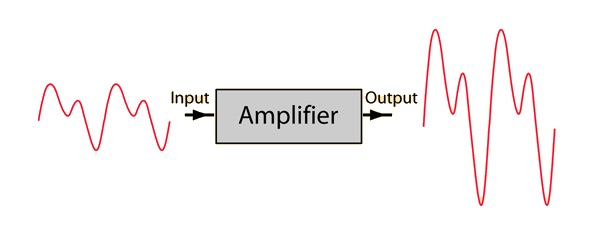
\includegraphics[width=4in]{amp}
  \caption{e.g. Amplifying a signal $y=5 x$}
\end{figure}
\end{frame}
%=-=-=-=-=-=-=-=-=-=-=-=-=-=-=-=-
\imageFrame{measure}{Measure it, also known as feature extraction.}
\imageFrame{audio}{How can we do that in more complex signals?}
\imageFrame{fourierPicture}{The Fourier Transformation (FT).}
\imageFrame{ft}{FT allows to identify frequency components upon complex signals.}
%Examples=-=-=-=-=-=-=-=-=-=-=-=-
\section{Examples of FT Applications}
\imageFrame{notchFT}{}
\imageFrame{qsr}{}
\imageFrame{image}{}
\imageFrame{xRayFT}{}
\imageFrame{tomography}{}
%Memes=--=-=-=-=-=-=-=-=-=-=-=-=-
\imageFrame{ftMeme}{}
%\imageFrame{ftMeme2}{}
%=-=-=-=-=-=-=-=-=-=-=-=-=-=-=-=-
%=-=-=-=-=-=-=-=-=-=-=-=-=-=-=-=-
%=-=-=-=-=-=-=-=-=-=-=-=-=-=-=-=-
%=-=-=-=-=-=-=-=-=-=-=-=-=-=-=-=-
%=-=-=-=-=-=-=-=-=-=-=-=-=-=-=-=-
\section{The Phonocardiogram Project}
\subsection{Basics of heart sound}
\begin{frame}{PhonoCardioGram (PCG)}
A PhonoCardioGram, also known as PCG, is a representation of
heart's audio signal ploted against time.

\begin{figure}
  \centering
  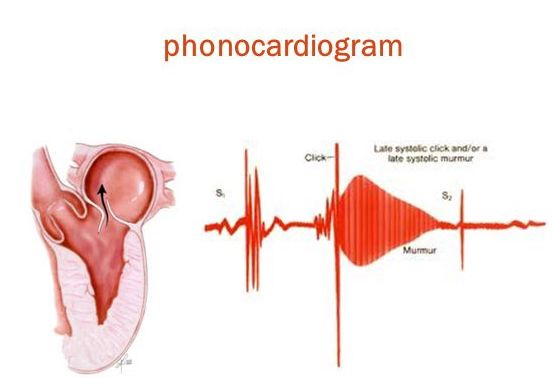
\includegraphics[width=3in]{pcg}
\end{figure}
\end{frame}
%=-=-=-=-=-=-=-=-=-=-=-=-=-=-=-=-
\begin{frame}{Which frequencies heart use to sing?}
In order to acquire the heart's audio signal, is important to know where
the heart's frequencies are.

\begin{figure}
  \centering
  
\includegraphics[width=2.5in]{singing}
\end{figure}
\end{frame}
%=-=-=-=-=-=-=-=-=-=-=-=-=-=-=-=-
\begin{frame}
\begin{figure}
  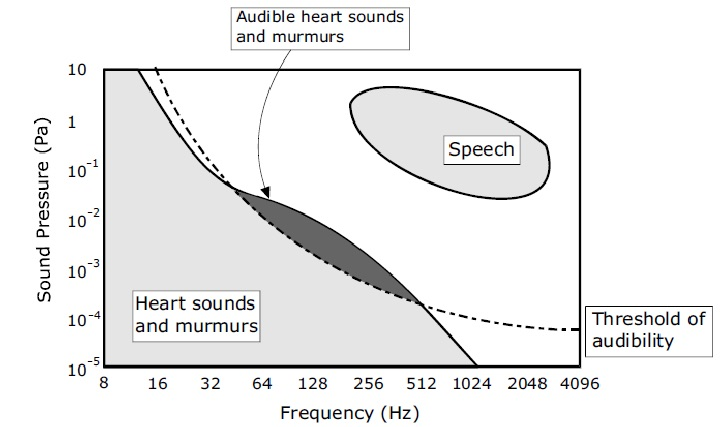
\includegraphics[width=4.5in]{heartFreq}
\end{figure}
\end{frame}
%=-=-=-=-=-=-=-=-=-=-=-=-=-=-=-=-
\section{Electronics Design Proposal}
%=-=-=-=-=-=-=-=-=-=-=-=-=-=-=-=-
\begin{frame}
\begin{figure}
  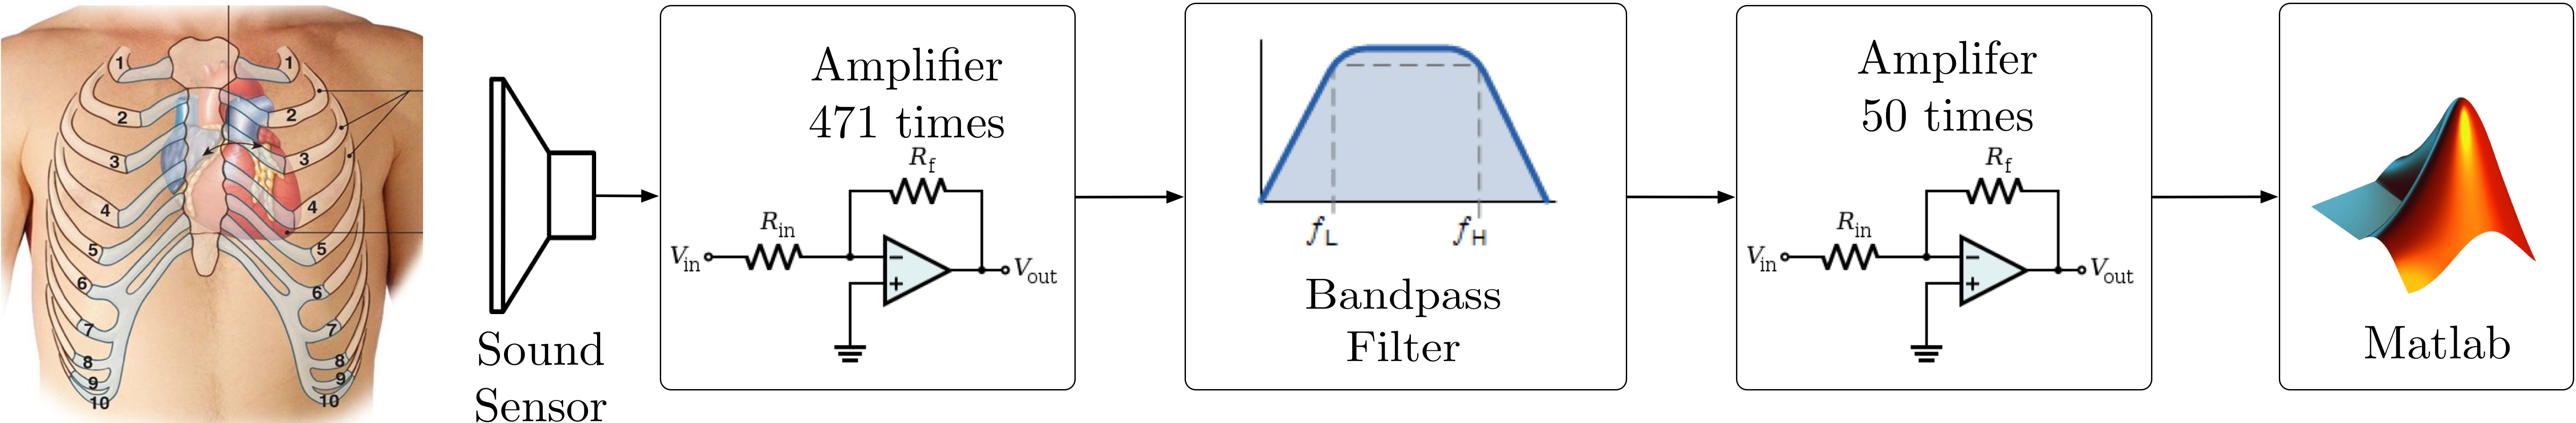
\includegraphics[width=4.5in]{pcgMethodology}
\end{figure}
\end{frame}
%%=-=-=-=-=-=-=-=-=-=-=-=-=-=-=-=-
\begin{frame}{Pre-Amp Stage}
\begin{figure}
  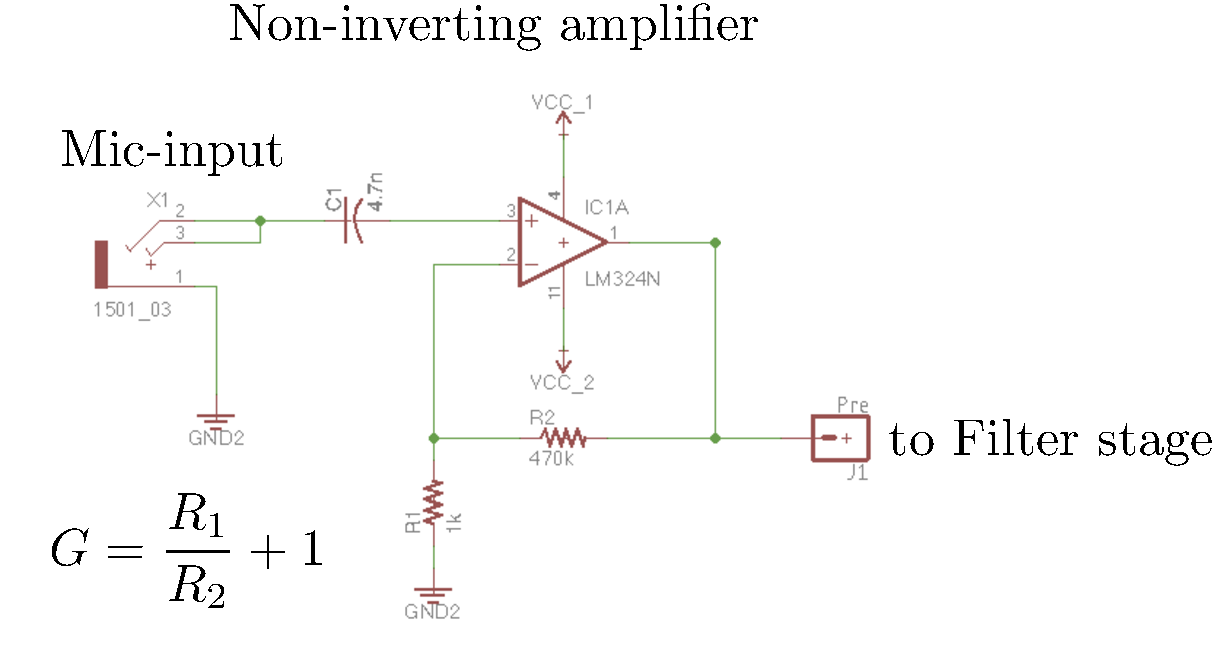
\includegraphics[width=4.5in]{preAmpStage}
\end{figure}
\end{frame}
%%=-=-=-=-=-=-=-=-=-=-=-=-=-=-=-=-
\begin{frame}{Band-pass}
\begin{figure}
  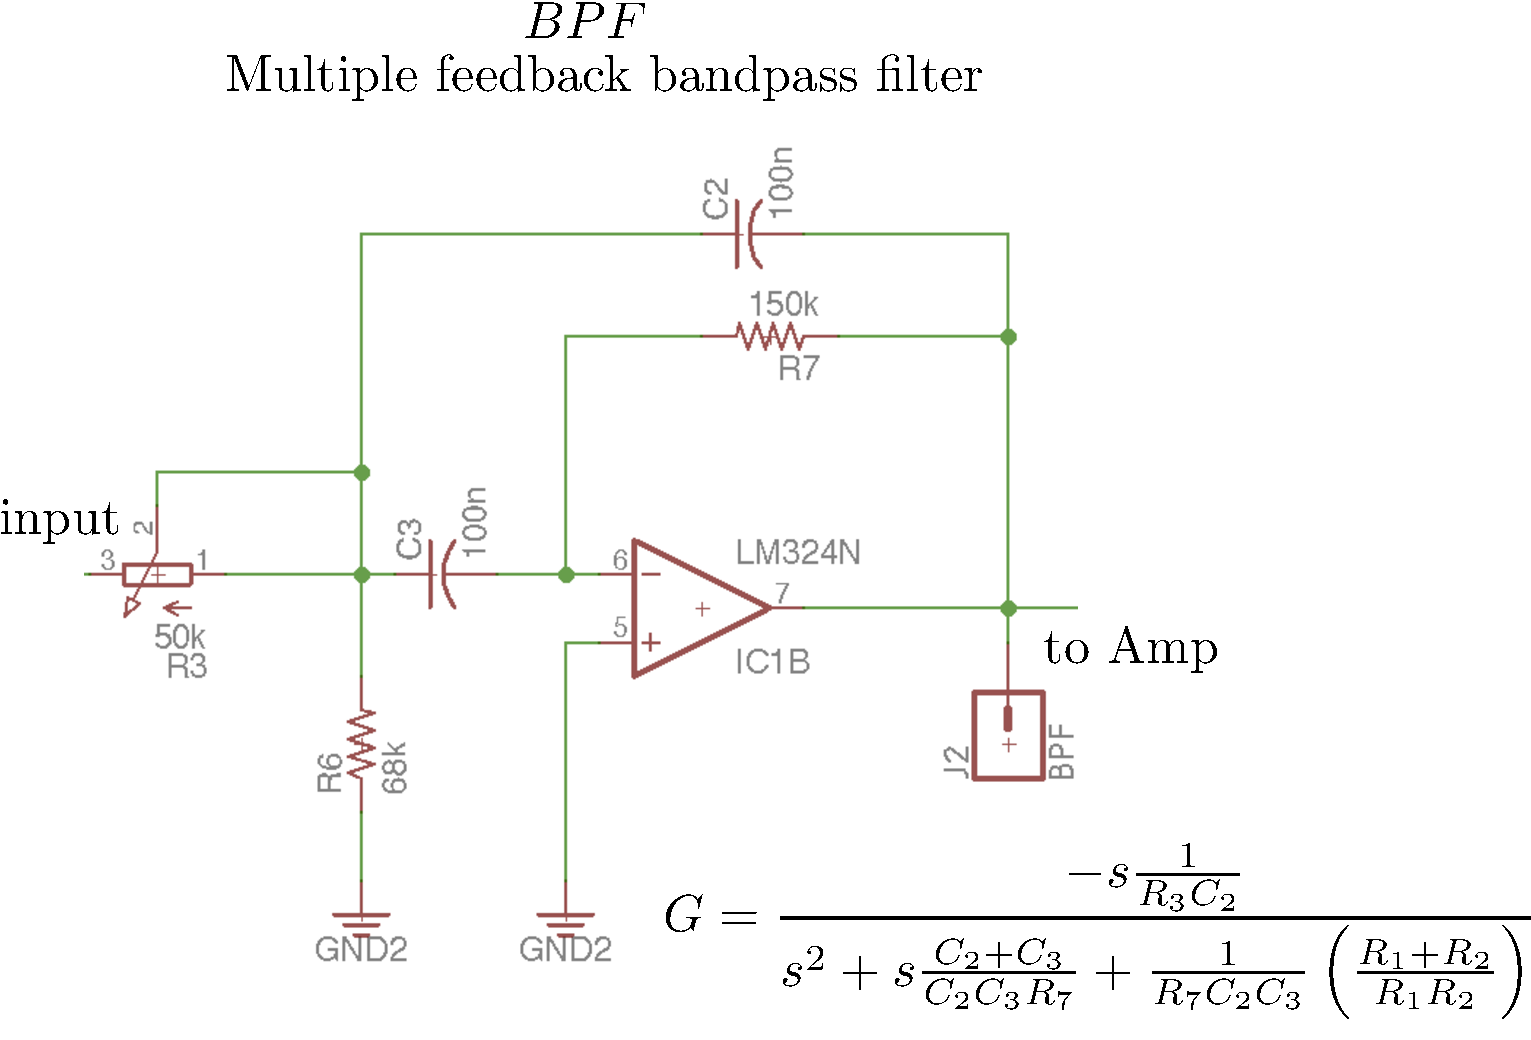
\includegraphics[width=4in]{bpfStage}
\end{figure}
\end{frame}
%%=-=-=-=-=-=-=-=-=-=-=-=-=-=-=-=-
\begin{frame}{Filter design}
The filter is defined by:
\begin{eqnarray*}
  k=2\pi f_0C_3\\
  C_2=C_3\\
  R_3=\frac{1}{Hk}\\
  R_6=\frac{1}{(2Q-H)k}\\
  R_5=\frac{2Q}{k}
\end{eqnarray*}
Design was tuned in:
\begin{eqnarray*}
  Q=2, f_0=33\\
  C_2=C_3=100nF\\
  H=2
\end{eqnarray*}

\end{frame}
%%=-=-=-=-=-=-=-=-=-=-=-=-=-=-=-=-
\begin{frame}{Filter's behaviour}
\begin{figure}
  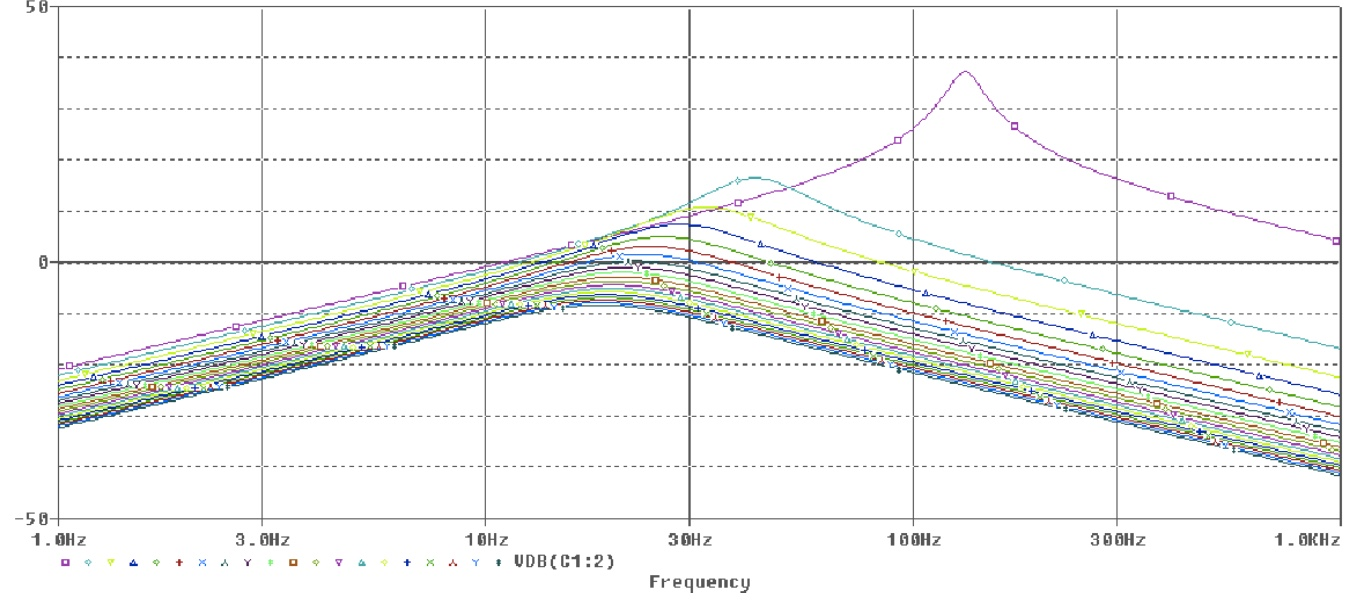
\includegraphics[width=4in]{filterBehaviour}
\end{figure}
\end{frame}
%%=-=-=-=-=-=-=-=-=-=-=-=-=-=-=-=-
%%=-=-=-=-=-=-=-=-=-=-=-=-=-=-=-=-
%%=-=-=-=-=-=-=-=-=-=-=-=-=-=-=-=-
%%=-=-=-=-=-=-=-=-=-=-=-=-=-=-=-=-
\begin{frame}{Inverting amplifier}
\begin{figure}
  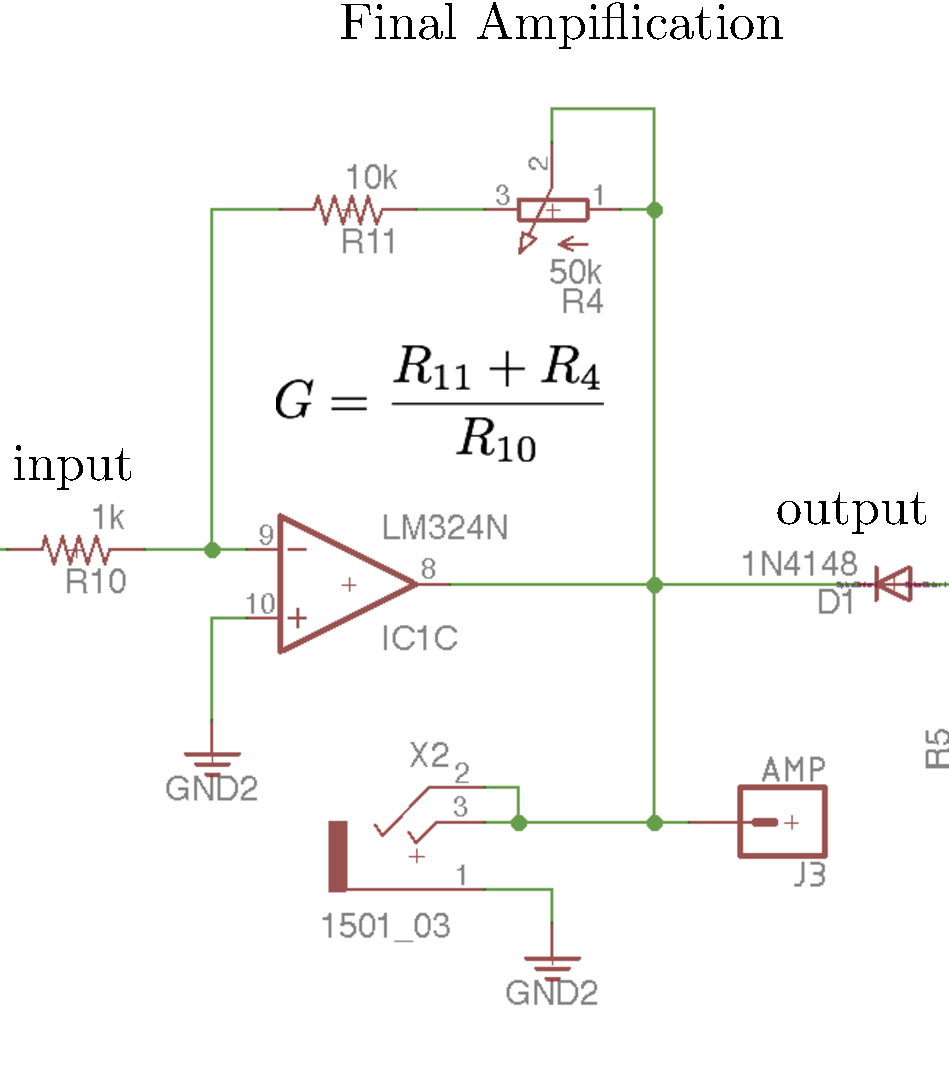
\includegraphics[height=3in]{ampStage}
\end{figure}
\end{frame}
%%=-=-=-=-=-=-=-=-=-=-=-=-=-=-=-=-
\imageFrame{eagle}{The IDE to create your own design}
%%=-=-=-=-=-=-=-=-=-=-=-=-=-=-=-=-
\imageFrame{pcbProcess}{Eagle, OrCAD, TINA, Altium, ...}
\imageFrame{homerLab}{Lets built our PCB}
%%=-=-=-=-=-=-=-=-=-=-=-=-=-=-=-=-
%%=-=-=-=-=-=-=-=-=-=-=-=-=-=-=-=-
%%=-=-=-=-=-=-=-=-=-=-=-=-=-=-=-=-
%%=-=-=-=-=-=-=-=-=-=-=-=-=-=-=-=-
%%=-=-=-=-=-=-=-=-=-=-=-=-=-=-=-=-
%%=-=-=-=-=-=-=-=-=-=-=-=-=-=-=-=-
%%=-=-=-=-=-=-=-=-=-=-=-=-=-=-=-=-


%
\begin{frame}
\begin{figure}
  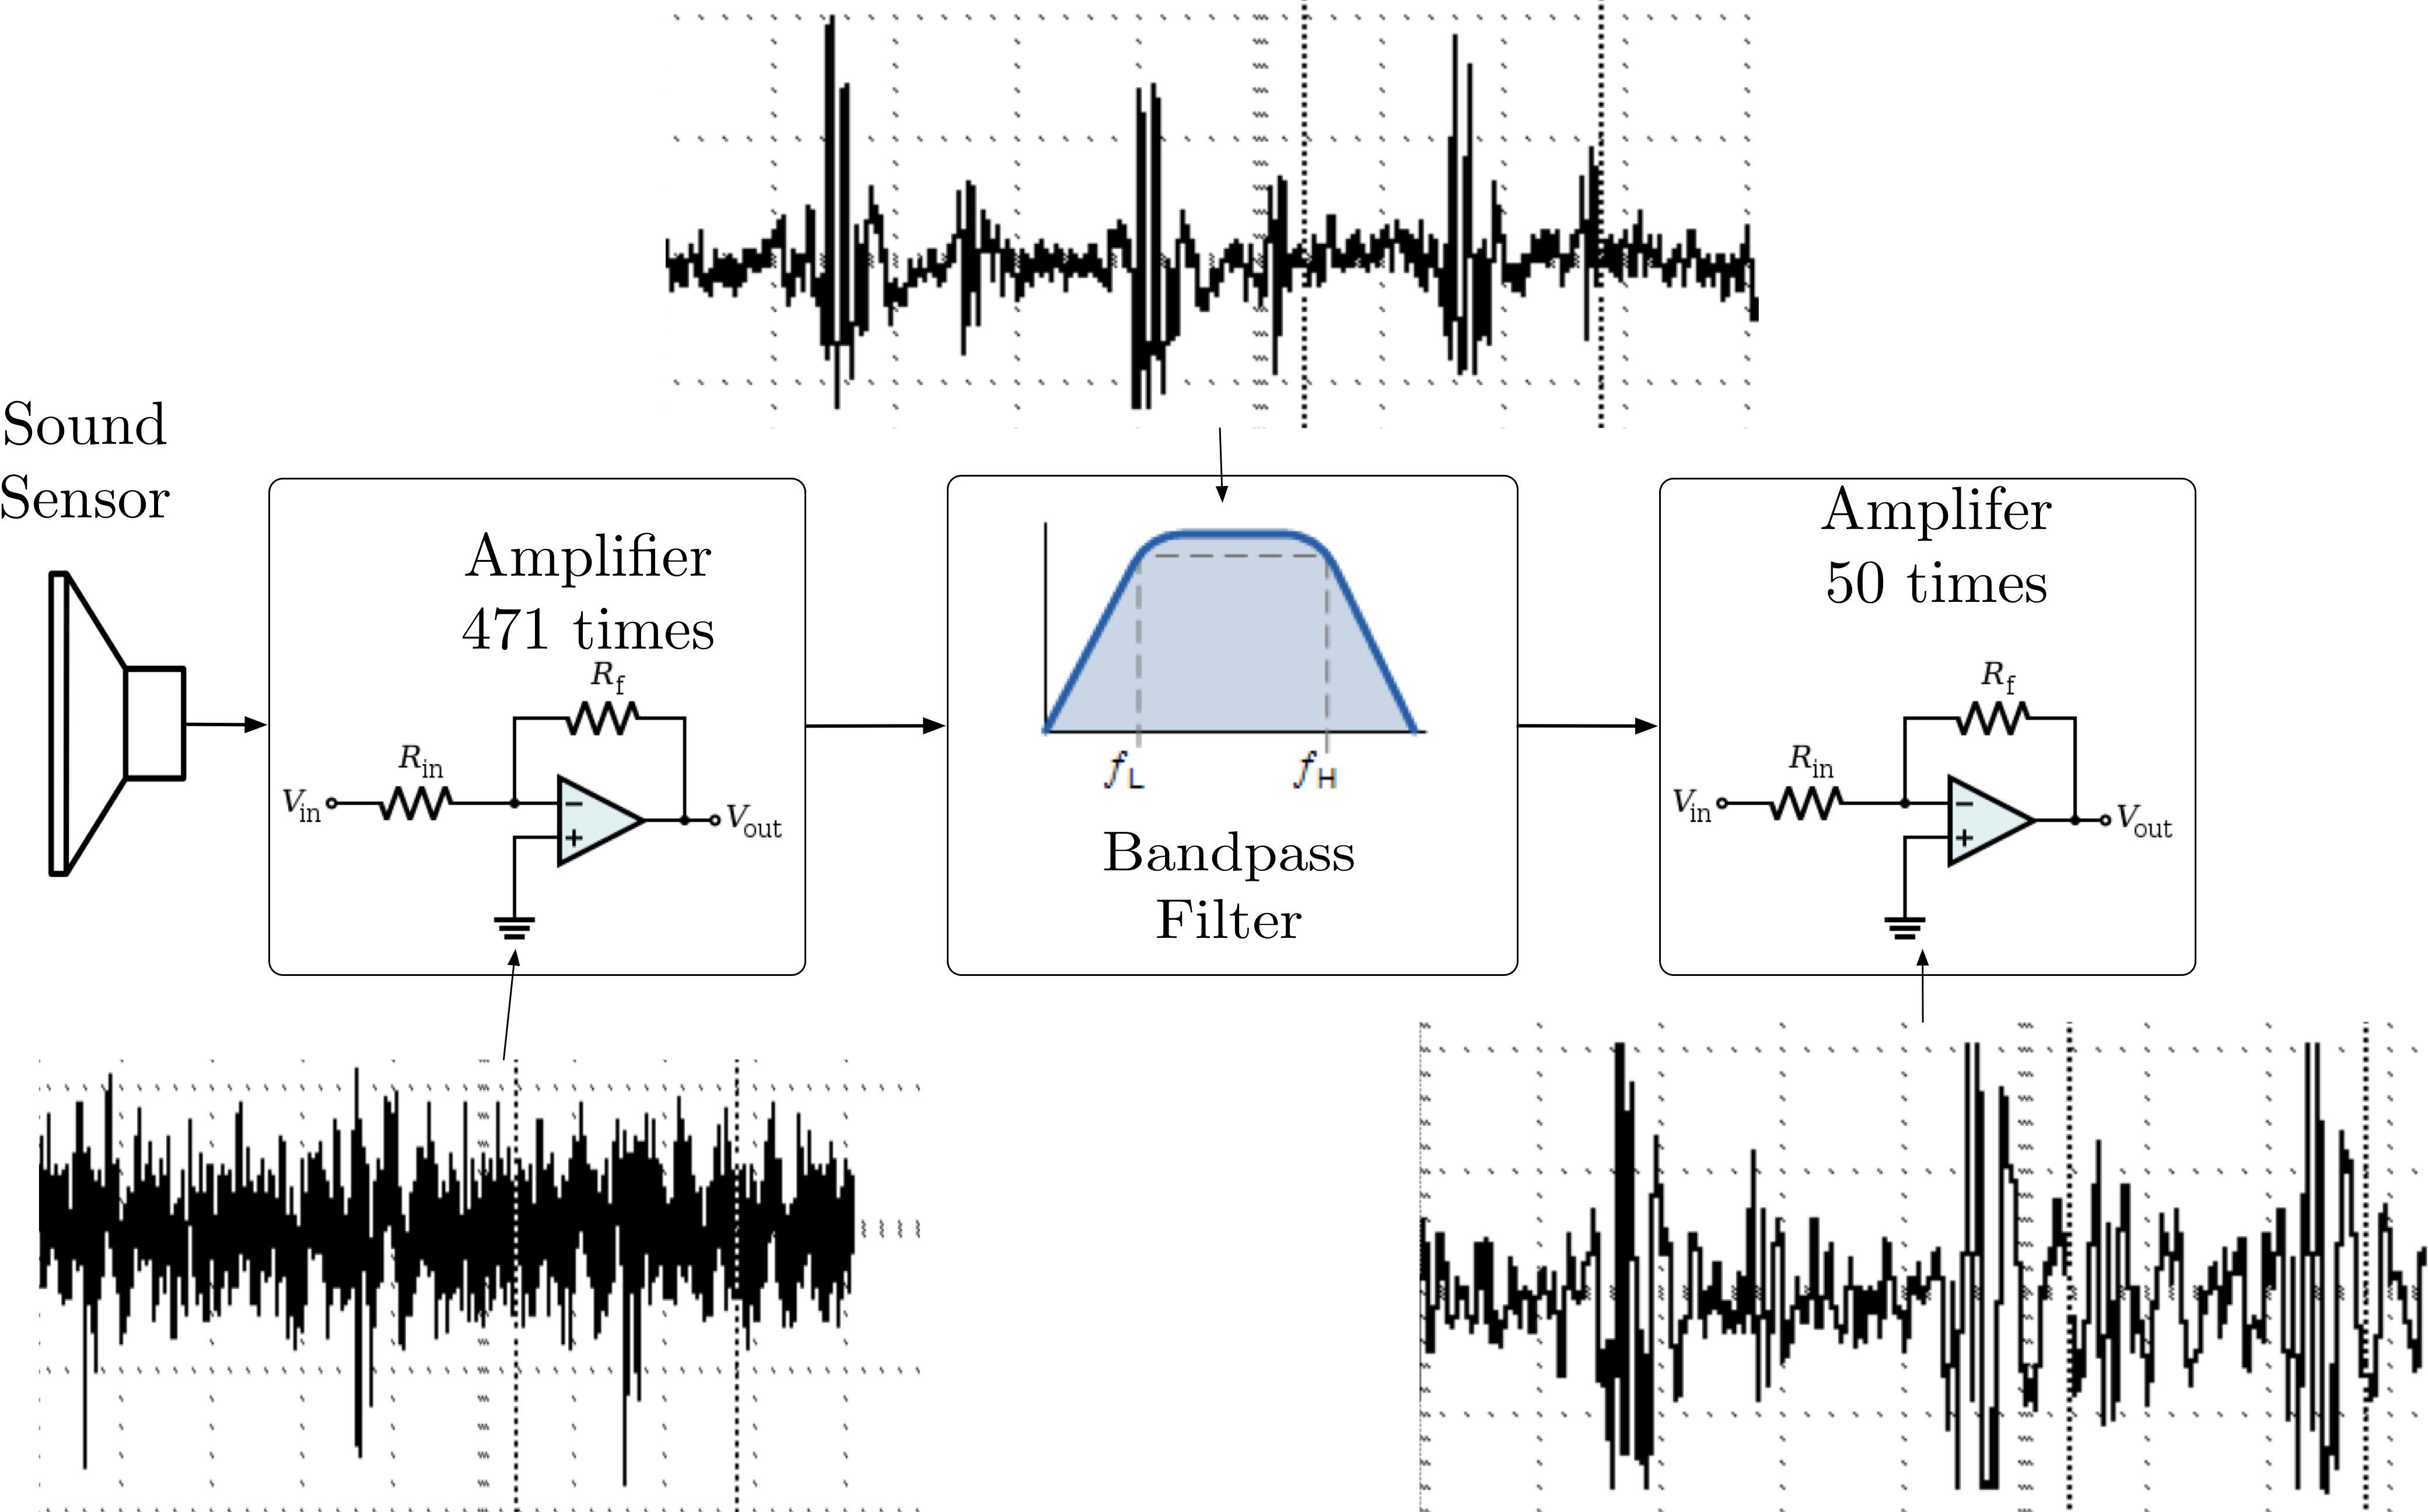
\includegraphics[width=4.5in]{pcgWaves}
\end{figure}
\end{frame}

%=-=-=-=-=-=-=-=-=-=-=-=-=-=-=-=-
%=-=-=-=-=-=-=-=-=-=-=-=-=-=-=-=-
%=-=-=-=-=-=-=-=-=-=-=-=-=-=-=-=-
%=-=-=-=-=-=-=-=-=-=-=-=-=-=-=-=-

%--------------------
\begin{frame}{References}
	\begin{thebibliography}{10}
	\beamertemplatebookbibitems

	\bibitem{Zill2009}
	Deniss G. Zill and Michael R. Cullen
	\newblock Differential Equations with Boundary-Valuer Problems,
	\newblock 7th Editions, 2009


	\beamertemplatebookbibitems
	\bibitem{Swokowski1983}
	Earl W. Swokowski
	\newblock Calculus with analytic geometry
	\newblock Prindle, Weber \& Schmidt, 1979

  \end{thebibliography}
\end{frame}
\end{document}
